\chapter{Lec 06 - Adversarial Search I}

\section{Adversarial Search}
Mathematical game theory, a branch of economics, views any multiagent environment as a game, provided that the impact of each agent on the others is “significant,” regardless of whether the agents are cooperative or competitive. In AI, the most common games are of a rather specialized kind, what game theorists call deterministic, turn-taking, two-player, zero-sum games of \textbf{perfect information} (such as chess). In our terminology, this means deterministic, fully observable environments in which two agents act alternately and in which the utility values at the end of the game are always equal and opposite. For example, if one player wins a game of chess, the other player necessarily loses. It is this opposition between the agents’ utility functions that makes the situation adversarial. There exist also \textbf{imperfect information} games, such as bridge, poker, scrabble, and games with non-deterministic outcomes, e.g. backgammon or monopoly.
\newline\newline
In a normal search problem, the optimal solution would be a sequence of actions leading to a goal state, a terminal state that is a win. In adversarial search, the solution is a strategy specifying a move for every possible opponent reply. Algorithms that deal with games also need to consider the time limits of the game itself (e.g. chess). Therefore, they require the ability to make some decision even when calculating the optimal decision is infeasible (approximation).\newline\newline
We first consider games with two players, whom we call MAX and MIN for reasons that will soon become obvious. MAX moves first, and then they take turns moving until the game is over. At the end of the game, points are awarded to the winning player and penalties are given to the loser.\newline\newline
The initial state, the legal moves in each state and the results of the moves form the so called \textbf{game tree}, where the nodes are game states and the edges are moves.
\begin{center}
    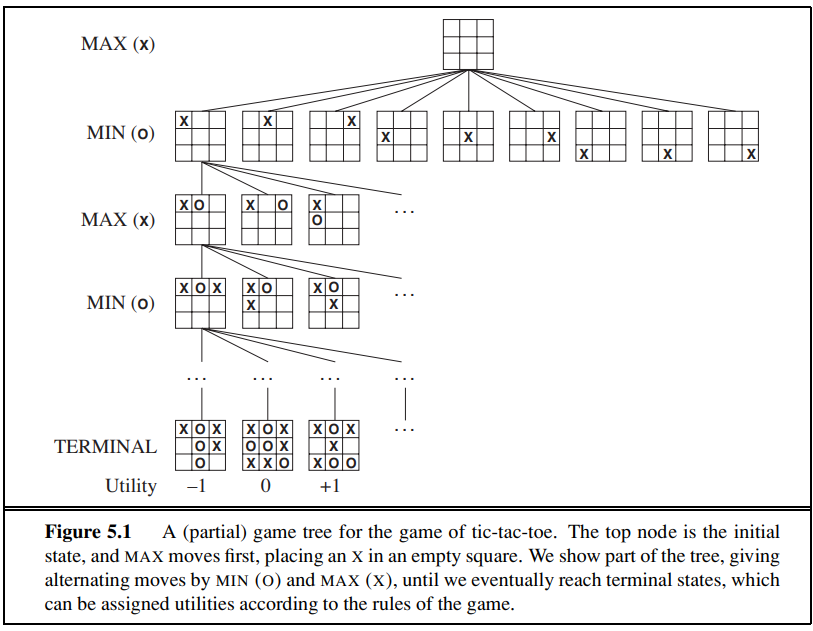
\includegraphics[scale=0.8]{images/tic-tac-toe.png}
\end{center}
The figure above shows part of the game tree for tic-tac-toe. From the initial state, MAX has nine possible moves. Play alternates between MAX’s placing an X and MIN’s placing an O until we reach leaf nodes corresponding to terminal states such that one player has three in a row or all the squares are filled.  The number on each leaf node indicates the \textbf{utility value} (provided by the \textbf{utility function}) of the terminal state; high values are assumed to be good for MAX and bad for MIN and viceversa. For tic-tac-toe the game tree is relatively small, fewer than $9! = 362,880$ terminal nodes. But for chess there are over $10^{40}$ nodes.\newline\newline
A utility function (also called an objective function or payoff function),
defines the final numeric value for a game that ends in terminal state $s$ for a player $p$. A \textbf{zero-sum} game is (confusingly) defined as one where the total payoff to all players is the same for every instance of the game. Chess is zero-sum because every game has payoff of either $0+1$, $1+0$ or $1/2 + 1/2$.

\section{Minimax}
Given a game tree, the optimal strategy can be determined from the \textbf{minimax} value of each node, which we write as MINIMAX($n$). The minimax value of a node is the utility (for MAX) of being in the corresponding state, \textbf{assuming that both players play optimally} from there to the end of the game. Obviously, the minimax value of a terminal state is just its utility.  Furthermore, given a choice, MAX prefers to move to a state of maximum value, whereas MIN prefers a state of minimum value. So we have the following:
\begin{center}
    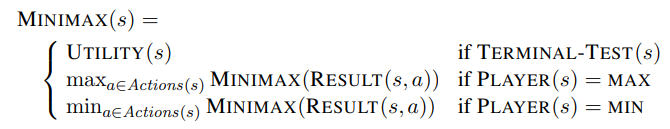
\includegraphics[]{images/minimax.png}
\end{center}
This definition of optimal play for MAX assumes that MIN also plays \textbf{optimally}, it maximizes the worst-case outcome for MAX. What if MIN does not play optimally? Then, it is easy to show that MAX will do even better. Other strategies against suboptimal opponents may do better than the minimax strategy, but these strategies necessarily do worse against optimal opponents.
\begin{center}
    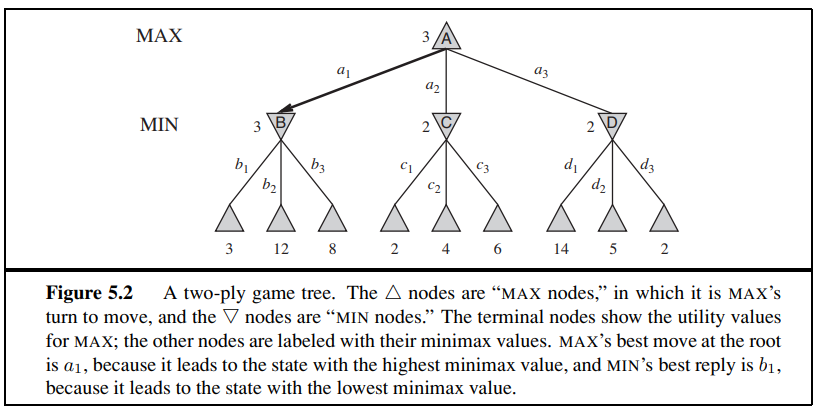
\includegraphics[]{images/minimax-game tree.png}
\end{center}
The \textbf{minimax algorithm} computes the minimax decision from the current state. It uses a simple recursive computation of the minimax values of each successor state. The recursion proceeds all the way down to the leaves of the tree, and then the minimax values are backed up through the tree as the recursion unwinds.
\begin{center}
    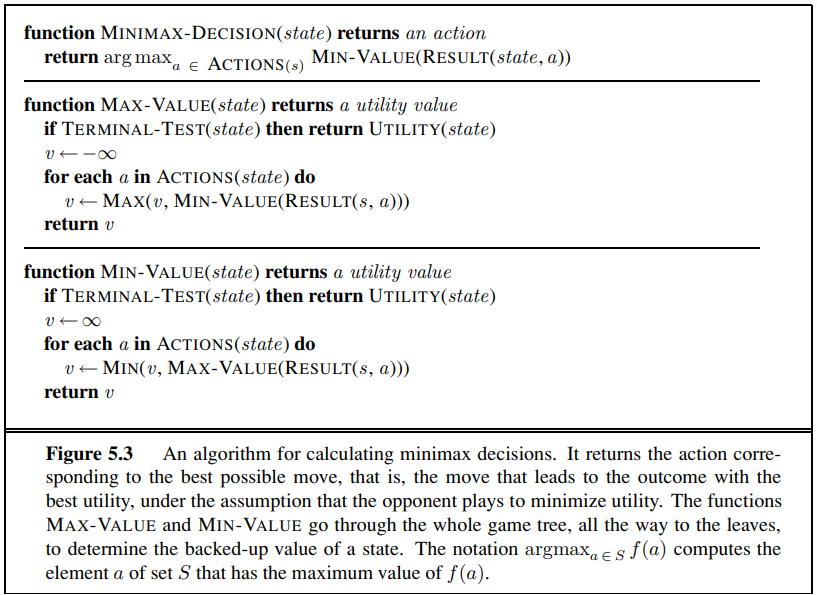
\includegraphics[]{images/minimax-algorithms.png}
\end{center}
The minimax algorithm performs a complete depth-first exploration of the game tree. If the maximum depth of the tree is $m$ and there are $b$ legal moves at each point, then the time complexity is $O(b^m)$. The space complexity is $O(bm)$. For real games, of course, the time cost is totally impractical, but this algorithm serves as the basis for the mathematical analysis of games and for more practical algorithms.

\section{Alpha-Beta Pruning}
The problem with minimax search is that the number of game states it has to examine is exponential in the depth of the tree. Unfortunately, we can’t eliminate the exponent, but it turns out we can effectively cut it in half. The trick is that it is possible to compute the \textbf{correct} minimax decision without looking at every node in the game tree. This particular technique  is called \textbf{alpha–beta pruning}.
\begin{center}
    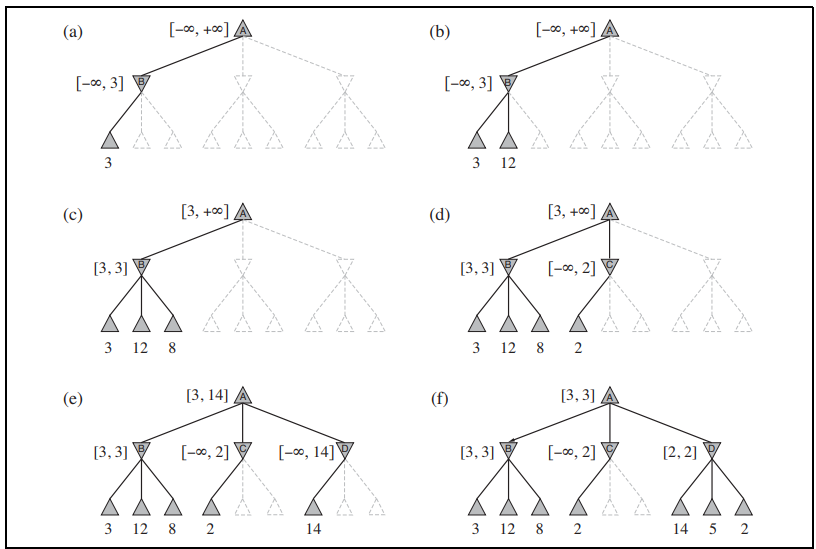
\includegraphics[]{images/alpha-beta pruning.png}
\end{center}
Alpha–beta pruning gets its name from the following two parameters that describe bounds on the backed-up values that appear anywhere along the path:
\begin{itemize}
    \item $\alpha = $ the value of the best (i.e., highest-value) choice we have found so far at any choice point along the path for MAX.

    \item $\beta = $ the value of the best (i.e., lowest-value) choice we have found so far at any choice point along the path for MIN.
\end{itemize}
Alpha–beta search updates the values of $\alpha$ and $\beta$ as it goes along and prunes the remaining branches at a node (i.e., terminates the recursive call) as soon as the value of the current node is known to be worse than the current $\alpha$ or $\beta$ value for MAX or MIN, respectively.
\begin{center}
    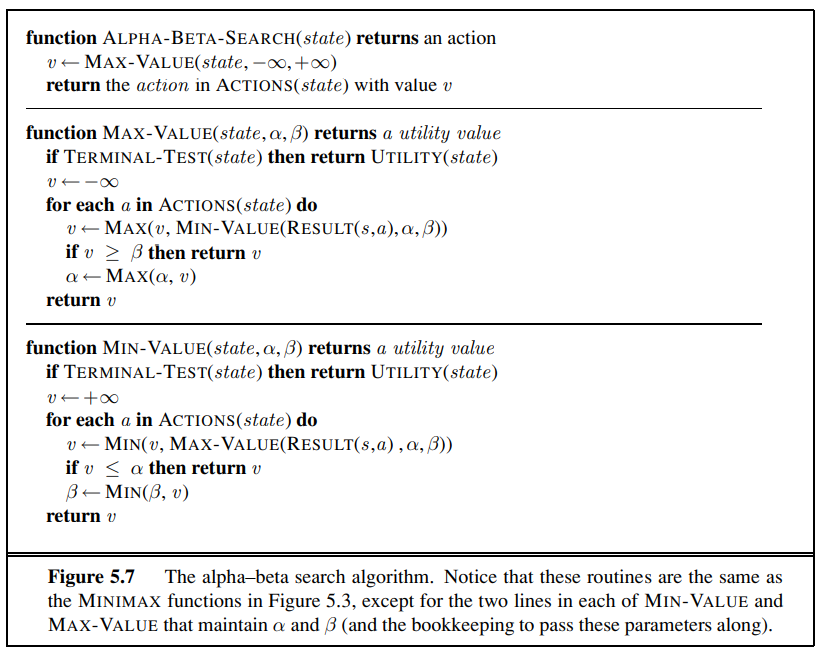
\includegraphics[]{images/a-b algo.png}
\end{center}
The effectiveness of alpha–beta pruning is highly dependent on the order in which the states are examined. A “good” ordering of the moves improves the effectiveness of pruning. In particular, the perfect order would be:
\begin{itemize}
    \item for MAX: from highest to lowest values;
    \item for MIN:  from lowest to highest values.
\end{itemize}
In this way, when MIN needs to examine its successors he knows that as soon as he founds a state with lower value than $\alpha$, he can prune the remaining nodes (the same is valid for MAX). With perfect order it turns out that alpha–beta needs to examine only $O(b^{m/2})$ nodes to pick the best move (which means we can double the search depth).
